%!TEX root = ../thesis.tex

\chapter{Practical performences}
\label{chap:pracPerf}

\section{\adaB}
\label{subsec:AdaPracPerf}
In an attempt to demonstrate the practical performance we recreated the following situation from \cite{Hastie2009}. We have ten features $X_1,\ldots,X_{10}$ which are drawn from a standard independent Gaussian. Their label is determined (deterministically) by the following rule: $$Y:=\begin{cases}
1 & \sum_{i=0}^{10} X^2_i > \chi_{10}^2(0.5)\\
0 & \text{otherwise}
\end{cases}$$ Where $\chi_{10}^2(0.5)=9.34$ is the median of a chi-squared random variable with ten degrees of freedom. The results of testing can be found in figure \ref{fig:adaB} and will be discussed below. 

\begin{figure}[!ht]
  \centering
      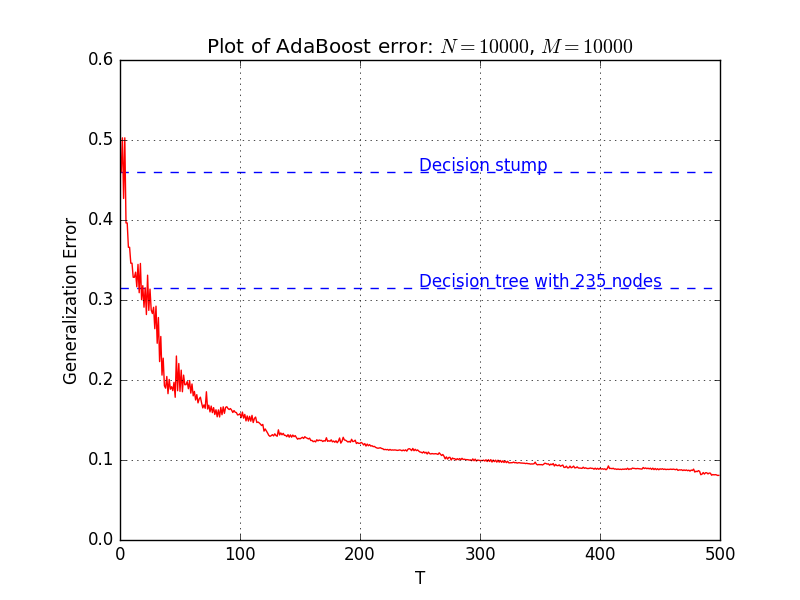
\includegraphics[width=0.8\textwidth]{generated/prettyLong.png}
  \caption{Generalization error of AdaBoost as a function of the number of iterations with 10000 examples and test cases. The error of actual stumps and a tree with 217 nodes is also shown for reference.}
      \label{fig:adaB}
\end{figure}

First of all it should be noted that we took an equal number of training and testing examples (10000 to be exact). This was possible because we can generate the data ourselves in a reasonable amount of time. In practical settings this is however usually not the case and one would need to reserve a portion of the data for testing instead of training. This means that the more testing one does, the less training one can do and thus, generally one would reserve only around 10\% of the data for testing.
\par Looking at figure \ref{fig:adaB} it is obvious that our algorithm works. The decision stump initially performs with an error rate of 47\% which is indeed only slightly better than random guessing. \adaB outperforms this and even a large tree with 217 nodes and an error rate of 30\% after just tens of iterations and reaches an error rate as low as 8\% after 400 iterations. 

 \section{\NHB}
 \label{subsec:NHPracPerf}